\documentclass[twoside]{book}

% Packages required by doxygen
\usepackage{calc}
\usepackage{doxygen}
\usepackage{graphicx}
\usepackage[utf8]{inputenc}
\usepackage{makeidx}
\usepackage{multicol}
\usepackage{multirow}
\usepackage{textcomp}
\usepackage[table]{xcolor}

% Font selection
\usepackage[T1]{fontenc}
\usepackage{mathptmx}
\usepackage[scaled=.90]{helvet}
\usepackage{courier}
\usepackage{amssymb}
\usepackage{sectsty}
\renewcommand{\familydefault}{\sfdefault}
\allsectionsfont{%
  \fontseries{bc}\selectfont%
  \color{darkgray}%
}
\renewcommand{\DoxyLabelFont}{%
  \fontseries{bc}\selectfont%
  \color{darkgray}%
}

% Page & text layout
\usepackage{geometry}
\geometry{%
  a4paper,%
  top=2.5cm,%
  bottom=2.5cm,%
  left=2.5cm,%
  right=2.5cm%
}
\tolerance=750
\hfuzz=15pt
\hbadness=750
\setlength{\emergencystretch}{15pt}
\setlength{\parindent}{0cm}
\setlength{\parskip}{0.2cm}
\makeatletter
\renewcommand{\paragraph}{%
  \@startsection{paragraph}{4}{0ex}{-1.0ex}{1.0ex}{%
    \normalfont\normalsize\bfseries\SS@parafont%
  }%
}
\renewcommand{\subparagraph}{%
  \@startsection{subparagraph}{5}{0ex}{-1.0ex}{1.0ex}{%
    \normalfont\normalsize\bfseries\SS@subparafont%
  }%
}
\makeatother

% Headers & footers
\usepackage{fancyhdr}
\pagestyle{fancyplain}
\fancyhead[LE]{\fancyplain{}{\bfseries\thepage}}
\fancyhead[CE]{\fancyplain{}{}}
\fancyhead[RE]{\fancyplain{}{\bfseries\leftmark}}
\fancyhead[LO]{\fancyplain{}{\bfseries\rightmark}}
\fancyhead[CO]{\fancyplain{}{}}
\fancyhead[RO]{\fancyplain{}{\bfseries\thepage}}
\fancyfoot[LE]{\fancyplain{}{}}
\fancyfoot[CE]{\fancyplain{}{}}
\fancyfoot[RE]{\fancyplain{}{\bfseries\scriptsize Generated on Fri May 19 2017 08\-:12\-:24 for Crisis\-Defender by Doxygen }}
\fancyfoot[LO]{\fancyplain{}{\bfseries\scriptsize Generated on Fri May 19 2017 08\-:12\-:24 for Crisis\-Defender by Doxygen }}
\fancyfoot[CO]{\fancyplain{}{}}
\fancyfoot[RO]{\fancyplain{}{}}
\renewcommand{\footrulewidth}{0.4pt}
\renewcommand{\chaptermark}[1]{%
  \markboth{#1}{}%
}
\renewcommand{\sectionmark}[1]{%
  \markright{\thesection\ #1}%
}

% Indices & bibliography
\usepackage{natbib}
\usepackage[titles]{tocloft}
\setcounter{tocdepth}{3}
\setcounter{secnumdepth}{5}
\makeindex

% Hyperlinks (required, but should be loaded last)
\usepackage{ifpdf}
\ifpdf
  \usepackage[pdftex,pagebackref=true]{hyperref}
\else
  \usepackage[ps2pdf,pagebackref=true]{hyperref}
\fi
\hypersetup{%
  colorlinks=true,%
  linkcolor=blue,%
  citecolor=blue,%
  unicode%
}

% Custom commands
\newcommand{\clearemptydoublepage}{%
  \newpage{\pagestyle{empty}\cleardoublepage}%
}


%===== C O N T E N T S =====

\begin{document}

% Titlepage & ToC
\hypersetup{pageanchor=false}
\pagenumbering{roman}
\begin{titlepage}
\vspace*{7cm}
\begin{center}%
{\Large Crisis\-Defender }\\
\vspace*{1cm}
{\large Generated by Doxygen 1.8.5}\\
\vspace*{0.5cm}
{\small Fri May 19 2017 08:12:24}\\
\end{center}
\end{titlepage}
\clearemptydoublepage
\tableofcontents
\clearemptydoublepage
\pagenumbering{arabic}
\hypersetup{pageanchor=true}

%--- Begin generated contents ---
\chapter{R\-E\-A\-D\-M\-E}
\label{md__r_e_a_d_m_e}
\hypertarget{md__r_e_a_d_m_e}{}
Crisis Defender, a topdown action arcade game. Alex Cowell, i7460122

Please put your resolution in config.\-txt (for example 1080) as one number (and no letters). Please be aware that the game will render out in a 16\-:9 ratio from your number, although you may resize the window if necessary. 
\chapter{Hierarchical Index}
\section{Class Hierarchy}
This inheritance list is sorted roughly, but not completely, alphabetically\-:\begin{DoxyCompactList}
\item \contentsline{section}{background}{\pageref{classbackground}}{}
\item \contentsline{section}{enemies}{\pageref{structenemies}}{}
\item \contentsline{section}{Enemy}{\pageref{class_enemy}}{}
\item \contentsline{section}{Heart}{\pageref{class_heart}}{}
\item \contentsline{section}{Player}{\pageref{class_player}}{}
\item Q\-Open\-G\-L\-Window\begin{DoxyCompactList}
\item \contentsline{section}{N\-G\-L\-Scene}{\pageref{class_n_g_l_scene}}{}
\end{DoxyCompactList}
\item \contentsline{section}{Sword}{\pageref{class_sword}}{}
\item \contentsline{section}{Win\-Params}{\pageref{struct_win_params}}{}
\end{DoxyCompactList}

\chapter{Class Index}
\section{Class List}
Here are the classes, structs, unions and interfaces with brief descriptions\-:\begin{DoxyCompactList}
\item\contentsline{section}{\hyperlink{classbackground}{background} }{\pageref{classbackground}}{}
\item\contentsline{section}{\hyperlink{structenemies}{enemies} \\*Struct for enemy data }{\pageref{structenemies}}{}
\item\contentsline{section}{\hyperlink{class_enemy}{Enemy} }{\pageref{class_enemy}}{}
\item\contentsline{section}{\hyperlink{class_heart}{Heart} }{\pageref{class_heart}}{}
\item\contentsline{section}{\hyperlink{class_n_g_l_scene}{N\-G\-L\-Scene} }{\pageref{class_n_g_l_scene}}{}
\item\contentsline{section}{\hyperlink{class_player}{Player} }{\pageref{class_player}}{}
\item\contentsline{section}{\hyperlink{class_sword}{Sword} }{\pageref{class_sword}}{}
\item\contentsline{section}{\hyperlink{struct_win_params}{Win\-Params} }{\pageref{struct_win_params}}{}
\end{DoxyCompactList}

\chapter{File Index}
\section{File List}
Here is a list of all documented files with brief descriptions\-:\begin{DoxyCompactList}
\item\contentsline{section}{include/\hyperlink{background_8h}{background.\-h} \\*Used for the background sphere }{\pageref{background_8h}}{}
\item\contentsline{section}{include/\hyperlink{_enemy_8h}{Enemy.\-h} \\*For the enemies }{\pageref{_enemy_8h}}{}
\item\contentsline{section}{include/\hyperlink{_heart_8h}{Heart.\-h} \\*For the heart health pickup }{\pageref{_heart_8h}}{}
\item\contentsline{section}{include/{\bfseries N\-G\-L\-Scene.\-h} }{\pageref{_n_g_l_scene_8h}}{}
\item\contentsline{section}{include/\hyperlink{_player_8h}{Player.\-h} \\*This is for the player character }{\pageref{_player_8h}}{}
\item\contentsline{section}{include/\hyperlink{_sword_8h}{Sword.\-h} \\*\hyperlink{class_sword}{Sword} object }{\pageref{_sword_8h}}{}
\item\contentsline{section}{include/\hyperlink{_window_params_8h}{Window\-Params.\-h} \\*For the windows }{\pageref{_window_params_8h}}{}
\end{DoxyCompactList}

\chapter{Class Documentation}
\hypertarget{classbackground}{\section{background Class Reference}
\label{classbackground}\index{background@{background}}
}
\subsection*{Public Member Functions}
\begin{DoxyCompactItemize}
\item 
\hyperlink{classbackground_ac312ccf8c912f5865f4b2f8a539151c7}{background} (std\-::string \-\_\-texture, std\-::string \-\_\-texture2)
\begin{DoxyCompactList}\small\item\em ctor \end{DoxyCompactList}\item 
\hypertarget{classbackground_a3eb375d1a5594efbd0a6c1a8dac439cd}{\hyperlink{classbackground_a3eb375d1a5594efbd0a6c1a8dac439cd}{$\sim$background} ()}\label{classbackground_a3eb375d1a5594efbd0a6c1a8dac439cd}

\begin{DoxyCompactList}\small\item\em dtor \end{DoxyCompactList}\item 
void \hyperlink{classbackground_aa79fc05bb4348453d625537efb8f0460}{draw} (ngl\-::\-Camera $\ast$\-\_\-cam)
\begin{DoxyCompactList}\small\item\em draw method \end{DoxyCompactList}\end{DoxyCompactItemize}


\subsection{Constructor \& Destructor Documentation}
\hypertarget{classbackground_ac312ccf8c912f5865f4b2f8a539151c7}{\index{background@{background}!background@{background}}
\index{background@{background}!background@{background}}
\subsubsection[{background}]{\setlength{\rightskip}{0pt plus 5cm}background\-::background (
\begin{DoxyParamCaption}
\item[{std\-::string}]{\-\_\-texture, }
\item[{std\-::string}]{\-\_\-texture2}
\end{DoxyParamCaption}
)}}\label{classbackground_ac312ccf8c912f5865f4b2f8a539151c7}


ctor 


\begin{DoxyParams}{Parameters}
{\em \-\_\-texture/\-\_\-texture2} & the texture to load in \\
\hline
\end{DoxyParams}


\subsection{Member Function Documentation}
\hypertarget{classbackground_aa79fc05bb4348453d625537efb8f0460}{\index{background@{background}!draw@{draw}}
\index{draw@{draw}!background@{background}}
\subsubsection[{draw}]{\setlength{\rightskip}{0pt plus 5cm}void background\-::draw (
\begin{DoxyParamCaption}
\item[{ngl\-::\-Camera $\ast$}]{\-\_\-cam}
\end{DoxyParamCaption}
)}}\label{classbackground_aa79fc05bb4348453d625537efb8f0460}


draw method 


\begin{DoxyParams}{Parameters}
{\em \-\_\-cam} & camera data \\
\hline
\end{DoxyParams}


The documentation for this class was generated from the following files\-:\begin{DoxyCompactItemize}
\item 
include/\hyperlink{background_8h}{background.\-h}\item 
src/background.\-cpp\end{DoxyCompactItemize}

\hypertarget{structenemies}{\section{enemies Struct Reference}
\label{structenemies}\index{enemies@{enemies}}
}


struct for enemy data  




{\ttfamily \#include $<$Enemy.\-h$>$}

\subsection*{Public Attributes}
\begin{DoxyCompactItemize}
\item 
\hypertarget{structenemies_afd54ed444c64332f99b6b2f05748c00a}{ngl\-::\-Vec3 \hyperlink{structenemies_afd54ed444c64332f99b6b2f05748c00a}{m\-\_\-pos}}\label{structenemies_afd54ed444c64332f99b6b2f05748c00a}

\begin{DoxyCompactList}\small\item\em position vector \end{DoxyCompactList}\item 
\hypertarget{structenemies_a1b20a27575599cab0d3296b89e43a11e}{int \hyperlink{structenemies_a1b20a27575599cab0d3296b89e43a11e}{health} = 1}\label{structenemies_a1b20a27575599cab0d3296b89e43a11e}

\begin{DoxyCompactList}\small\item\em a value for enemy health \end{DoxyCompactList}\item 
\hypertarget{structenemies_a53f400db7f025d1aa7ade848adf7a127}{ngl\-::\-Transformation \hyperlink{structenemies_a53f400db7f025d1aa7ade848adf7a127}{m\-\_\-transform}}\label{structenemies_a53f400db7f025d1aa7ade848adf7a127}

\begin{DoxyCompactList}\small\item\em a transform stack \end{DoxyCompactList}\item 
\hypertarget{structenemies_ae8ebc70fc81a14f7706e6ded0a42e657}{float \hyperlink{structenemies_ae8ebc70fc81a14f7706e6ded0a42e657}{m\-\_\-rotation}}\label{structenemies_ae8ebc70fc81a14f7706e6ded0a42e657}

\begin{DoxyCompactList}\small\item\em the enemy's rotation \end{DoxyCompactList}\item 
\hypertarget{structenemies_aec12e728bbf6e02ca4fa7ac54dbab8d1}{std\-::unique\-\_\-ptr$<$ ngl\-::\-Obj $>$ \hyperlink{structenemies_aec12e728bbf6e02ca4fa7ac54dbab8d1}{m\-\_\-mesh}}\label{structenemies_aec12e728bbf6e02ca4fa7ac54dbab8d1}

\begin{DoxyCompactList}\small\item\em the enemy mesh \end{DoxyCompactList}\end{DoxyCompactItemize}


\subsection{Detailed Description}
struct for enemy data 

The documentation for this struct was generated from the following file\-:\begin{DoxyCompactItemize}
\item 
include/\hyperlink{_enemy_8h}{Enemy.\-h}\end{DoxyCompactItemize}

\hypertarget{class_enemy}{\section{Enemy Class Reference}
\label{class_enemy}\index{Enemy@{Enemy}}
}
\subsection*{Public Member Functions}
\begin{DoxyCompactItemize}
\item 
\hyperlink{class_enemy_a2d1b1a14c8df3df8b230c1ae38e1e193}{Enemy} (ngl\-::\-Vec3 \-\_\-pos, std\-::string \-\_\-fname)
\begin{DoxyCompactList}\small\item\em ctor \end{DoxyCompactList}\item 
void \hyperlink{class_enemy_ae7e82c8a3afd8b39ab3947fa1ece3394}{draw} (const std\-::string \&\-\_\-shader, ngl\-::\-Camera $\ast$\-\_\-cam)
\begin{DoxyCompactList}\small\item\em draw method \end{DoxyCompactList}\item 
void \hyperlink{class_enemy_a1a3c17dff184c23dfcc1f4ec499f7b36}{move\-Enemy} (ngl\-::\-Vec3 spos)
\begin{DoxyCompactList}\small\item\em movement method \end{DoxyCompactList}\item 
int \hyperlink{class_enemy_ab572397c421fd9dda7491360d53741ca}{attack} (ngl\-::\-Vec3 spos, int rot)
\begin{DoxyCompactList}\small\item\em enemy being attacked method \end{DoxyCompactList}\item 
int \hyperlink{class_enemy_a83b9d3f2d42c6abc0a9759fb59cd93b5}{knockback\-Player} (ngl\-::\-Vec3 spos)
\begin{DoxyCompactList}\small\item\em method to work out player/enemy collision and knockback \end{DoxyCompactList}\item 
\hypertarget{class_enemy_a533fe9819e7a304caaa51938590a49ff}{void \hyperlink{class_enemy_a533fe9819e7a304caaa51938590a49ff}{enemy\-Collisions} ()}\label{class_enemy_a533fe9819e7a304caaa51938590a49ff}

\begin{DoxyCompactList}\small\item\em enemy collision method \end{DoxyCompactList}\end{DoxyCompactItemize}
\subsection*{Public Attributes}
\begin{DoxyCompactItemize}
\item 
\hypertarget{class_enemy_ad20c260afb7bb563f05c9c86b451d058}{std\-::vector$<$ \hyperlink{structenemies}{enemies} $>$ \hyperlink{class_enemy_ad20c260afb7bb563f05c9c86b451d058}{m\-\_\-enemies}}\label{class_enemy_ad20c260afb7bb563f05c9c86b451d058}

\begin{DoxyCompactList}\small\item\em vector of enemy structs \end{DoxyCompactList}\item 
\hypertarget{class_enemy_a98766d083fc49e746a37d0dc69be09e0}{float \hyperlink{class_enemy_a98766d083fc49e746a37d0dc69be09e0}{speed} = 0.\-1}\label{class_enemy_a98766d083fc49e746a37d0dc69be09e0}

\begin{DoxyCompactList}\small\item\em movement speed variable \end{DoxyCompactList}\end{DoxyCompactItemize}


\subsection{Constructor \& Destructor Documentation}
\hypertarget{class_enemy_a2d1b1a14c8df3df8b230c1ae38e1e193}{\index{Enemy@{Enemy}!Enemy@{Enemy}}
\index{Enemy@{Enemy}!Enemy@{Enemy}}
\subsubsection[{Enemy}]{\setlength{\rightskip}{0pt plus 5cm}Enemy\-::\-Enemy (
\begin{DoxyParamCaption}
\item[{ngl\-::\-Vec3}]{\-\_\-pos, }
\item[{std\-::string}]{\-\_\-fname}
\end{DoxyParamCaption}
)}}\label{class_enemy_a2d1b1a14c8df3df8b230c1ae38e1e193}


ctor 


\begin{DoxyParams}{Parameters}
{\em \-\_\-pos} & the initial position \\
\hline
{\em \-\_\-fname} & the name of mesh to load \\
\hline
\end{DoxyParams}


\subsection{Member Function Documentation}
\hypertarget{class_enemy_ab572397c421fd9dda7491360d53741ca}{\index{Enemy@{Enemy}!attack@{attack}}
\index{attack@{attack}!Enemy@{Enemy}}
\subsubsection[{attack}]{\setlength{\rightskip}{0pt plus 5cm}int Enemy\-::attack (
\begin{DoxyParamCaption}
\item[{ngl\-::\-Vec3}]{spos, }
\item[{int}]{rot}
\end{DoxyParamCaption}
)}}\label{class_enemy_ab572397c421fd9dda7491360d53741ca}


enemy being attacked method 


\begin{DoxyParams}{Parameters}
{\em spos} & player position \\
\hline
{\em rot} & player facing direction \\
\hline
\end{DoxyParams}
\hypertarget{class_enemy_ae7e82c8a3afd8b39ab3947fa1ece3394}{\index{Enemy@{Enemy}!draw@{draw}}
\index{draw@{draw}!Enemy@{Enemy}}
\subsubsection[{draw}]{\setlength{\rightskip}{0pt plus 5cm}void Enemy\-::draw (
\begin{DoxyParamCaption}
\item[{const std\-::string \&}]{\-\_\-shader, }
\item[{ngl\-::\-Camera $\ast$}]{\-\_\-cam}
\end{DoxyParamCaption}
)}}\label{class_enemy_ae7e82c8a3afd8b39ab3947fa1ece3394}


draw method 


\begin{DoxyParams}{Parameters}
{\em \-\_\-shader} & the shader to use \\
\hline
{\em \-\_\-cam} & camera data passed on \\
\hline
\end{DoxyParams}
\hypertarget{class_enemy_a83b9d3f2d42c6abc0a9759fb59cd93b5}{\index{Enemy@{Enemy}!knockback\-Player@{knockback\-Player}}
\index{knockback\-Player@{knockback\-Player}!Enemy@{Enemy}}
\subsubsection[{knockback\-Player}]{\setlength{\rightskip}{0pt plus 5cm}int Enemy\-::knockback\-Player (
\begin{DoxyParamCaption}
\item[{ngl\-::\-Vec3}]{spos}
\end{DoxyParamCaption}
)}}\label{class_enemy_a83b9d3f2d42c6abc0a9759fb59cd93b5}


method to work out player/enemy collision and knockback 


\begin{DoxyParams}{Parameters}
{\em spos} & player position \\
\hline
\end{DoxyParams}
\hypertarget{class_enemy_a1a3c17dff184c23dfcc1f4ec499f7b36}{\index{Enemy@{Enemy}!move\-Enemy@{move\-Enemy}}
\index{move\-Enemy@{move\-Enemy}!Enemy@{Enemy}}
\subsubsection[{move\-Enemy}]{\setlength{\rightskip}{0pt plus 5cm}void Enemy\-::move\-Enemy (
\begin{DoxyParamCaption}
\item[{ngl\-::\-Vec3}]{spos}
\end{DoxyParamCaption}
)}}\label{class_enemy_a1a3c17dff184c23dfcc1f4ec499f7b36}


movement method 


\begin{DoxyParams}{Parameters}
{\em spos} & player's position passed on for chasing \\
\hline
\end{DoxyParams}


The documentation for this class was generated from the following files\-:\begin{DoxyCompactItemize}
\item 
include/\hyperlink{_enemy_8h}{Enemy.\-h}\item 
src/Enemy.\-cpp\end{DoxyCompactItemize}

\hypertarget{class_heart}{\section{Heart Class Reference}
\label{class_heart}\index{Heart@{Heart}}
}
\subsection*{Public Member Functions}
\begin{DoxyCompactItemize}
\item 
\hyperlink{class_heart_a10e7414c251624a7394c8e49ff7e6b92}{Heart} (ngl\-::\-Vec3 \-\_\-pos, std\-::string \-\_\-fname)
\begin{DoxyCompactList}\small\item\em ctor \end{DoxyCompactList}\item 
void \hyperlink{class_heart_a2a262356476149c5c08cd40cc0d6e762}{draw} (const std\-::string \&\-\_\-shader, ngl\-::\-Camera $\ast$\-\_\-cam)
\begin{DoxyCompactList}\small\item\em draw method \end{DoxyCompactList}\item 
bool \hyperlink{class_heart_a609cd2acaccbcd8230e9ce10d2c82ad9}{collide} (ngl\-::\-Vec3 spos)
\begin{DoxyCompactList}\small\item\em collision method \end{DoxyCompactList}\item 
\hypertarget{class_heart_a33fcca1d7d422d827924ef052636eb60}{bool \hyperlink{class_heart_a33fcca1d7d422d827924ef052636eb60}{spawn} ()}\label{class_heart_a33fcca1d7d422d827924ef052636eb60}

\begin{DoxyCompactList}\small\item\em method to determine whether it will spawn \end{DoxyCompactList}\end{DoxyCompactItemize}
\subsection*{Public Attributes}
\begin{DoxyCompactItemize}
\item 
\hypertarget{class_heart_a5b4ac61c0cceedc82cfc47ba5acbea4c}{ngl\-::\-Vec3 \hyperlink{class_heart_a5b4ac61c0cceedc82cfc47ba5acbea4c}{m\-\_\-pos}}\label{class_heart_a5b4ac61c0cceedc82cfc47ba5acbea4c}

\begin{DoxyCompactList}\small\item\em the position of the heart \end{DoxyCompactList}\end{DoxyCompactItemize}


\subsection{Constructor \& Destructor Documentation}
\hypertarget{class_heart_a10e7414c251624a7394c8e49ff7e6b92}{\index{Heart@{Heart}!Heart@{Heart}}
\index{Heart@{Heart}!Heart@{Heart}}
\subsubsection[{Heart}]{\setlength{\rightskip}{0pt plus 5cm}Heart\-::\-Heart (
\begin{DoxyParamCaption}
\item[{ngl\-::\-Vec3}]{\-\_\-pos, }
\item[{std\-::string}]{\-\_\-fname}
\end{DoxyParamCaption}
)}}\label{class_heart_a10e7414c251624a7394c8e49ff7e6b92}


ctor 


\begin{DoxyParams}{Parameters}
{\em \-\_\-pos} & the initial position \\
\hline
{\em \-\_\-fname} & the name of mesh to load \\
\hline
\end{DoxyParams}


\subsection{Member Function Documentation}
\hypertarget{class_heart_a609cd2acaccbcd8230e9ce10d2c82ad9}{\index{Heart@{Heart}!collide@{collide}}
\index{collide@{collide}!Heart@{Heart}}
\subsubsection[{collide}]{\setlength{\rightskip}{0pt plus 5cm}bool Heart\-::collide (
\begin{DoxyParamCaption}
\item[{ngl\-::\-Vec3}]{spos}
\end{DoxyParamCaption}
)}}\label{class_heart_a609cd2acaccbcd8230e9ce10d2c82ad9}


collision method 


\begin{DoxyParams}{Parameters}
{\em spos} & player position \\
\hline
\end{DoxyParams}
\hypertarget{class_heart_a2a262356476149c5c08cd40cc0d6e762}{\index{Heart@{Heart}!draw@{draw}}
\index{draw@{draw}!Heart@{Heart}}
\subsubsection[{draw}]{\setlength{\rightskip}{0pt plus 5cm}void Heart\-::draw (
\begin{DoxyParamCaption}
\item[{const std\-::string \&}]{\-\_\-shader, }
\item[{ngl\-::\-Camera $\ast$}]{\-\_\-cam}
\end{DoxyParamCaption}
)}}\label{class_heart_a2a262356476149c5c08cd40cc0d6e762}


draw method 


\begin{DoxyParams}{Parameters}
{\em \-\_\-shader} & the shader to use \\
\hline
{\em \-\_\-cam} & camera data passed on \\
\hline
\end{DoxyParams}


The documentation for this class was generated from the following files\-:\begin{DoxyCompactItemize}
\item 
include/\hyperlink{_heart_8h}{Heart.\-h}\item 
src/Heart.\-cpp\end{DoxyCompactItemize}

\hypertarget{class_n_g_l_scene}{\section{N\-G\-L\-Scene Class Reference}
\label{class_n_g_l_scene}\index{N\-G\-L\-Scene@{N\-G\-L\-Scene}}
}
Inheritance diagram for N\-G\-L\-Scene\-:\begin{figure}[H]
\begin{center}
\leavevmode
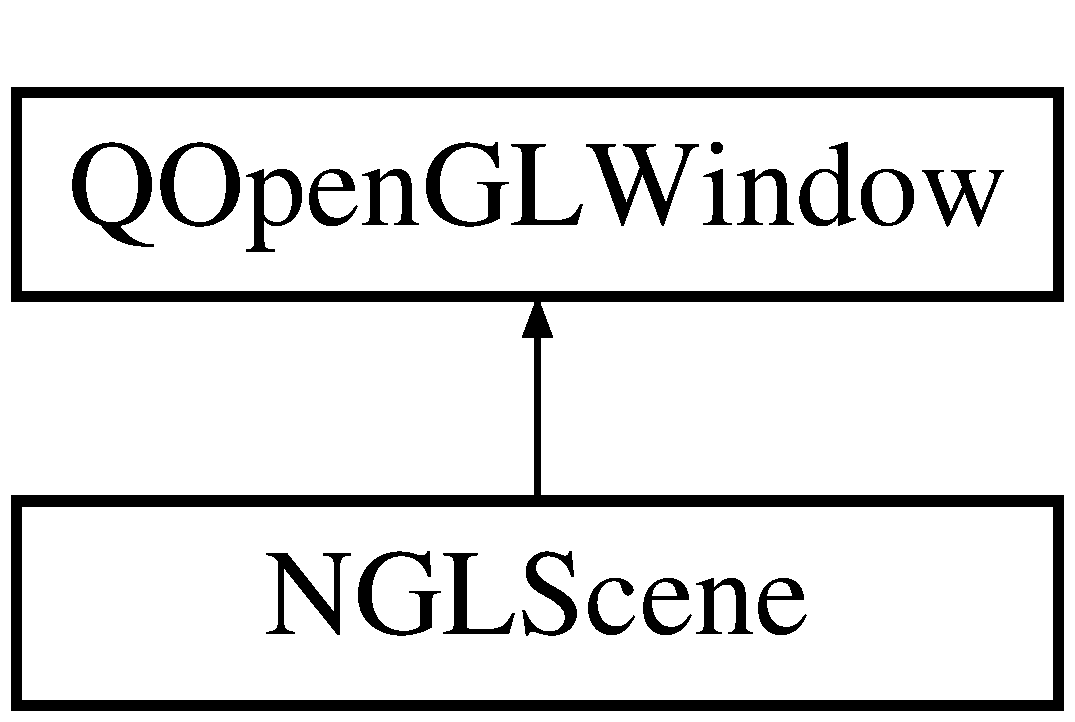
\includegraphics[height=2.000000cm]{class_n_g_l_scene}
\end{center}
\end{figure}
\subsection*{Public Member Functions}
\begin{DoxyCompactItemize}
\item 
\hypertarget{class_n_g_l_scene_a1bed6be9823459aeb1e58af2464ba633}{\hyperlink{class_n_g_l_scene_a1bed6be9823459aeb1e58af2464ba633}{N\-G\-L\-Scene} ()}\label{class_n_g_l_scene_a1bed6be9823459aeb1e58af2464ba633}

\begin{DoxyCompactList}\small\item\em ctor for our N\-G\-L drawing class \end{DoxyCompactList}\item 
\hypertarget{class_n_g_l_scene_abda05d130945833bfbb6bad8d619f7f5}{\hyperlink{class_n_g_l_scene_abda05d130945833bfbb6bad8d619f7f5}{$\sim$\-N\-G\-L\-Scene} ()}\label{class_n_g_l_scene_abda05d130945833bfbb6bad8d619f7f5}

\begin{DoxyCompactList}\small\item\em dtor must close down ngl and release Open\-G\-L resources \end{DoxyCompactList}\item 
\hypertarget{class_n_g_l_scene_aab2b866db534d286a56cc2240ed98790}{void \hyperlink{class_n_g_l_scene_aab2b866db534d286a56cc2240ed98790}{initialize\-G\-L} ()}\label{class_n_g_l_scene_aab2b866db534d286a56cc2240ed98790}

\begin{DoxyCompactList}\small\item\em the initialize class is called once when the window is created and we have a valid G\-L context use this to setup any default G\-L stuff \end{DoxyCompactList}\item 
\hypertarget{class_n_g_l_scene_a37bec65bfba7b7a717d803d369221e2d}{void \hyperlink{class_n_g_l_scene_a37bec65bfba7b7a717d803d369221e2d}{paint\-G\-L} ()}\label{class_n_g_l_scene_a37bec65bfba7b7a717d803d369221e2d}

\begin{DoxyCompactList}\small\item\em this is called everytime we want to draw the scene \end{DoxyCompactList}\item 
\hypertarget{class_n_g_l_scene_a7505fac688fe82b4f99e601043eb7764}{void \hyperlink{class_n_g_l_scene_a7505fac688fe82b4f99e601043eb7764}{resize\-G\-L} (int \-\_\-w, int \-\_\-h)}\label{class_n_g_l_scene_a7505fac688fe82b4f99e601043eb7764}

\begin{DoxyCompactList}\small\item\em this is called everytime we resize \end{DoxyCompactList}\end{DoxyCompactItemize}


The documentation for this class was generated from the following files\-:\begin{DoxyCompactItemize}
\item 
include/N\-G\-L\-Scene.\-h\item 
src/N\-G\-L\-Scene.\-cpp\end{DoxyCompactItemize}

\hypertarget{class_player}{\section{Player Class Reference}
\label{class_player}\index{Player@{Player}}
}
\subsection*{Public Member Functions}
\begin{DoxyCompactItemize}
\item 
\hyperlink{class_player_aefda42632e28f032d83750890da0fb26}{Player} (ngl\-::\-Vec3 \-\_\-pos, std\-::string \-\_\-fname)
\begin{DoxyCompactList}\small\item\em ctor \end{DoxyCompactList}\item 
void \hyperlink{class_player_afa7a7c657b9ab9f7bd342db96c1608af}{draw} (const std\-::string \&\-\_\-shader, ngl\-::\-Camera $\ast$\-\_\-cam)
\begin{DoxyCompactList}\small\item\em draw method \end{DoxyCompactList}\item 
void \hyperlink{class_player_a564e56488765c3fd7216698c415d9431}{move} (float \-\_\-x, float \-\_\-y)
\begin{DoxyCompactList}\small\item\em move method \end{DoxyCompactList}\end{DoxyCompactItemize}
\subsection*{Public Attributes}
\begin{DoxyCompactItemize}
\item 
\hypertarget{class_player_abe61d516fab1c2baec12586e93907811}{ngl\-::\-Vec3 \hyperlink{class_player_abe61d516fab1c2baec12586e93907811}{m\-\_\-pos}}\label{class_player_abe61d516fab1c2baec12586e93907811}

\begin{DoxyCompactList}\small\item\em the position of the player \end{DoxyCompactList}\item 
\hypertarget{class_player_aad33b52bfe73c4c978a3135172f286a0}{int \hyperlink{class_player_aad33b52bfe73c4c978a3135172f286a0}{health} = 3}\label{class_player_aad33b52bfe73c4c978a3135172f286a0}

\begin{DoxyCompactList}\small\item\em player health value \end{DoxyCompactList}\item 
\hypertarget{class_player_acd5f8e9953ff8d643954f425e2a0b197}{float \hyperlink{class_player_acd5f8e9953ff8d643954f425e2a0b197}{m\-\_\-rotation}}\label{class_player_acd5f8e9953ff8d643954f425e2a0b197}

\begin{DoxyCompactList}\small\item\em rotation value \end{DoxyCompactList}\item 
\hypertarget{class_player_ace6abae8d66534ad0a1fd6458f786a6e}{int \hyperlink{class_player_ace6abae8d66534ad0a1fd6458f786a6e}{score} = 0}\label{class_player_ace6abae8d66534ad0a1fd6458f786a6e}

\begin{DoxyCompactList}\small\item\em score value \end{DoxyCompactList}\item 
\hypertarget{class_player_a102fffbd6250cb9c776d2b8ff98b51ca}{int \hyperlink{class_player_a102fffbd6250cb9c776d2b8ff98b51ca}{mult} = 1}\label{class_player_a102fffbd6250cb9c776d2b8ff98b51ca}

\begin{DoxyCompactList}\small\item\em multiplier value \end{DoxyCompactList}\end{DoxyCompactItemize}


\subsection{Constructor \& Destructor Documentation}
\hypertarget{class_player_aefda42632e28f032d83750890da0fb26}{\index{Player@{Player}!Player@{Player}}
\index{Player@{Player}!Player@{Player}}
\subsubsection[{Player}]{\setlength{\rightskip}{0pt plus 5cm}Player\-::\-Player (
\begin{DoxyParamCaption}
\item[{ngl\-::\-Vec3}]{\-\_\-pos, }
\item[{std\-::string}]{\-\_\-fname}
\end{DoxyParamCaption}
)}}\label{class_player_aefda42632e28f032d83750890da0fb26}


ctor 


\begin{DoxyParams}{Parameters}
{\em \-\_\-pos} & the initial position \\
\hline
{\em \-\_\-fname} & the name of mesh to load \\
\hline
\end{DoxyParams}


\subsection{Member Function Documentation}
\hypertarget{class_player_afa7a7c657b9ab9f7bd342db96c1608af}{\index{Player@{Player}!draw@{draw}}
\index{draw@{draw}!Player@{Player}}
\subsubsection[{draw}]{\setlength{\rightskip}{0pt plus 5cm}void Player\-::draw (
\begin{DoxyParamCaption}
\item[{const std\-::string \&}]{\-\_\-shader, }
\item[{ngl\-::\-Camera $\ast$}]{\-\_\-cam}
\end{DoxyParamCaption}
)}}\label{class_player_afa7a7c657b9ab9f7bd342db96c1608af}


draw method 


\begin{DoxyParams}{Parameters}
{\em \-\_\-shader} & the shader to use \\
\hline
{\em \-\_\-cam} & camera data passed on \\
\hline
\end{DoxyParams}
\hypertarget{class_player_a564e56488765c3fd7216698c415d9431}{\index{Player@{Player}!move@{move}}
\index{move@{move}!Player@{Player}}
\subsubsection[{move}]{\setlength{\rightskip}{0pt plus 5cm}void Player\-::move (
\begin{DoxyParamCaption}
\item[{float}]{\-\_\-x, }
\item[{float}]{\-\_\-y}
\end{DoxyParamCaption}
)}}\label{class_player_a564e56488765c3fd7216698c415d9431}


move method 


\begin{DoxyParams}{Parameters}
{\em \-\_\-x,\-\_\-y} & values to transform with \\
\hline
\end{DoxyParams}


The documentation for this class was generated from the following files\-:\begin{DoxyCompactItemize}
\item 
include/\hyperlink{_player_8h}{Player.\-h}\item 
src/Player.\-cpp\end{DoxyCompactItemize}

\hypertarget{class_sword}{\section{Sword Class Reference}
\label{class_sword}\index{Sword@{Sword}}
}
\subsection*{Public Member Functions}
\begin{DoxyCompactItemize}
\item 
\hyperlink{class_sword_af691a6e171248ecddf4a789b34babb2e}{Sword} (ngl\-::\-Vec3 \-\_\-pos, std\-::string \-\_\-fname)
\begin{DoxyCompactList}\small\item\em ctor \end{DoxyCompactList}\item 
void \hyperlink{class_sword_afc2461586ea51d11fa6efaccdaf988fe}{draw} (const std\-::string \&\-\_\-shader, ngl\-::\-Camera $\ast$\-\_\-cam)
\begin{DoxyCompactList}\small\item\em draw method \end{DoxyCompactList}\item 
void \hyperlink{class_sword_aae6a84368d81a6d20beb946ee7b403a8}{move} (ngl\-::\-Vec3 spos)
\begin{DoxyCompactList}\small\item\em move method \end{DoxyCompactList}\end{DoxyCompactItemize}
\subsection*{Public Attributes}
\begin{DoxyCompactItemize}
\item 
\hypertarget{class_sword_aee9c64dbc2060e74b35d8919ce5161f7}{ngl\-::\-Vec3 \hyperlink{class_sword_aee9c64dbc2060e74b35d8919ce5161f7}{m\-\_\-pos}}\label{class_sword_aee9c64dbc2060e74b35d8919ce5161f7}

\begin{DoxyCompactList}\small\item\em the position of the ship \end{DoxyCompactList}\item 
\hypertarget{class_sword_a6cb5db3d2d4927b0e0d3ad5ebc07606a}{float \hyperlink{class_sword_a6cb5db3d2d4927b0e0d3ad5ebc07606a}{m\-\_\-rotation}}\label{class_sword_a6cb5db3d2d4927b0e0d3ad5ebc07606a}

\begin{DoxyCompactList}\small\item\em the sword's rotation \end{DoxyCompactList}\end{DoxyCompactItemize}


\subsection{Constructor \& Destructor Documentation}
\hypertarget{class_sword_af691a6e171248ecddf4a789b34babb2e}{\index{Sword@{Sword}!Sword@{Sword}}
\index{Sword@{Sword}!Sword@{Sword}}
\subsubsection[{Sword}]{\setlength{\rightskip}{0pt plus 5cm}Sword\-::\-Sword (
\begin{DoxyParamCaption}
\item[{ngl\-::\-Vec3}]{\-\_\-pos, }
\item[{std\-::string}]{\-\_\-fname}
\end{DoxyParamCaption}
)}}\label{class_sword_af691a6e171248ecddf4a789b34babb2e}


ctor 


\begin{DoxyParams}{Parameters}
{\em \-\_\-pos} & the initial position \\
\hline
{\em \-\_\-fname} & the name of mesh to load \\
\hline
\end{DoxyParams}


\subsection{Member Function Documentation}
\hypertarget{class_sword_afc2461586ea51d11fa6efaccdaf988fe}{\index{Sword@{Sword}!draw@{draw}}
\index{draw@{draw}!Sword@{Sword}}
\subsubsection[{draw}]{\setlength{\rightskip}{0pt plus 5cm}void Sword\-::draw (
\begin{DoxyParamCaption}
\item[{const std\-::string \&}]{\-\_\-shader, }
\item[{ngl\-::\-Camera $\ast$}]{\-\_\-cam}
\end{DoxyParamCaption}
)}}\label{class_sword_afc2461586ea51d11fa6efaccdaf988fe}


draw method 


\begin{DoxyParams}{Parameters}
{\em \-\_\-shader} & the shader to use \\
\hline
{\em \-\_\-cam} & camera data passed on \\
\hline
\end{DoxyParams}
\hypertarget{class_sword_aae6a84368d81a6d20beb946ee7b403a8}{\index{Sword@{Sword}!move@{move}}
\index{move@{move}!Sword@{Sword}}
\subsubsection[{move}]{\setlength{\rightskip}{0pt plus 5cm}void Sword\-::move (
\begin{DoxyParamCaption}
\item[{ngl\-::\-Vec3}]{spos}
\end{DoxyParamCaption}
)}}\label{class_sword_aae6a84368d81a6d20beb946ee7b403a8}


move method 


\begin{DoxyParams}{Parameters}
{\em spos} & the position of the player \\
\hline
\end{DoxyParams}


The documentation for this class was generated from the following files\-:\begin{DoxyCompactItemize}
\item 
include/\hyperlink{_sword_8h}{Sword.\-h}\item 
src/Sword.\-cpp\end{DoxyCompactItemize}

\hypertarget{struct_win_params}{\section{Win\-Params Struct Reference}
\label{struct_win_params}\index{Win\-Params@{Win\-Params}}
}
\subsection*{Public Attributes}
\begin{DoxyCompactItemize}
\item 
\hypertarget{struct_win_params_ae834d382a91e06699778caf8abf8b6a0}{int \hyperlink{struct_win_params_ae834d382a91e06699778caf8abf8b6a0}{spin\-X\-Face} = 0}\label{struct_win_params_ae834d382a91e06699778caf8abf8b6a0}

\begin{DoxyCompactList}\small\item\em used to store the x rotation mouse value \end{DoxyCompactList}\item 
\hypertarget{struct_win_params_adf538a60ecec846bb85fb790cdf02ef6}{int \hyperlink{struct_win_params_adf538a60ecec846bb85fb790cdf02ef6}{spin\-Y\-Face} = 0}\label{struct_win_params_adf538a60ecec846bb85fb790cdf02ef6}

\begin{DoxyCompactList}\small\item\em used to store the y rotation mouse value \end{DoxyCompactList}\item 
\hypertarget{struct_win_params_a255e3c376110315e2a4ff63ccc312360}{bool \hyperlink{struct_win_params_a255e3c376110315e2a4ff63ccc312360}{rotate} = false}\label{struct_win_params_a255e3c376110315e2a4ff63ccc312360}

\begin{DoxyCompactList}\small\item\em flag to indicate if the mouse button is pressed when dragging \end{DoxyCompactList}\item 
\hypertarget{struct_win_params_adcfa86195240b478c94bfecc5e33e8e7}{bool \hyperlink{struct_win_params_adcfa86195240b478c94bfecc5e33e8e7}{translate} = false}\label{struct_win_params_adcfa86195240b478c94bfecc5e33e8e7}

\begin{DoxyCompactList}\small\item\em flag to indicate if the Right mouse button is pressed when dragging \end{DoxyCompactList}\item 
\hypertarget{struct_win_params_ab9ddf234ba11eb4460eb48469cd73c3a}{int \hyperlink{struct_win_params_ab9ddf234ba11eb4460eb48469cd73c3a}{orig\-X} = 0}\label{struct_win_params_ab9ddf234ba11eb4460eb48469cd73c3a}

\begin{DoxyCompactList}\small\item\em the previous x mouse value \end{DoxyCompactList}\item 
\hypertarget{struct_win_params_a9e4ef1b5ef96c1f6bbe46bb10c11d59b}{int \hyperlink{struct_win_params_a9e4ef1b5ef96c1f6bbe46bb10c11d59b}{orig\-Y} = 0}\label{struct_win_params_a9e4ef1b5ef96c1f6bbe46bb10c11d59b}

\begin{DoxyCompactList}\small\item\em the previous y mouse value \end{DoxyCompactList}\item 
\hypertarget{struct_win_params_ab07a11274084415333c1fd0a5fc03667}{int \hyperlink{struct_win_params_ab07a11274084415333c1fd0a5fc03667}{orig\-X\-Pos} = 0}\label{struct_win_params_ab07a11274084415333c1fd0a5fc03667}

\begin{DoxyCompactList}\small\item\em the previous x mouse value for Position changes \end{DoxyCompactList}\item 
\hypertarget{struct_win_params_a5dc76afc1f5486221ee40eee3cb9a5ac}{int \hyperlink{struct_win_params_a5dc76afc1f5486221ee40eee3cb9a5ac}{orig\-Y\-Pos} = 0}\label{struct_win_params_a5dc76afc1f5486221ee40eee3cb9a5ac}

\begin{DoxyCompactList}\small\item\em the previous y mouse value for Position changes \end{DoxyCompactList}\item 
\hypertarget{struct_win_params_abe7daa1f3fc56dc639141bcbee759c02}{int \hyperlink{struct_win_params_abe7daa1f3fc56dc639141bcbee759c02}{width} = 1920}\label{struct_win_params_abe7daa1f3fc56dc639141bcbee759c02}

\begin{DoxyCompactList}\small\item\em window width \end{DoxyCompactList}\item 
\hypertarget{struct_win_params_a9b7c0ae0270bc1f7cfad6d95524b886b}{int \hyperlink{struct_win_params_a9b7c0ae0270bc1f7cfad6d95524b886b}{height} = 1080}\label{struct_win_params_a9b7c0ae0270bc1f7cfad6d95524b886b}

\begin{DoxyCompactList}\small\item\em window height \end{DoxyCompactList}\end{DoxyCompactItemize}


The documentation for this struct was generated from the following file\-:\begin{DoxyCompactItemize}
\item 
include/\hyperlink{_window_params_8h}{Window\-Params.\-h}\end{DoxyCompactItemize}

\chapter{File Documentation}
\hypertarget{background_8h}{\section{include/background.h File Reference}
\label{background_8h}\index{include/background.\-h@{include/background.\-h}}
}


used for the background sphere  


{\ttfamily \#include $<$ngl/\-Camera.\-h$>$}\\*
{\ttfamily \#include $<$string$>$}\\*
\subsection*{Classes}
\begin{DoxyCompactItemize}
\item 
class \hyperlink{classbackground}{background}
\end{DoxyCompactItemize}


\subsection{Detailed Description}
used for the background sphere \begin{DoxyAuthor}{Author}
Alex Cowell 
\end{DoxyAuthor}

\hypertarget{_enemy_8h}{\section{include/\-Enemy.h File Reference}
\label{_enemy_8h}\index{include/\-Enemy.\-h@{include/\-Enemy.\-h}}
}


for the enemies  


{\ttfamily \#include $<$ngl/\-Camera.\-h$>$}\\*
{\ttfamily \#include $<$ngl/\-Vec3.\-h$>$}\\*
{\ttfamily \#include $<$ngl/\-Obj.\-h$>$}\\*
{\ttfamily \#include $<$ngl/\-Transformation.\-h$>$}\\*
\subsection*{Classes}
\begin{DoxyCompactItemize}
\item 
struct \hyperlink{structenemies}{enemies}
\begin{DoxyCompactList}\small\item\em struct for enemy data \end{DoxyCompactList}\item 
class \hyperlink{class_enemy}{Enemy}
\end{DoxyCompactItemize}


\subsection{Detailed Description}
for the enemies this class inherits from the Qt Open\-G\-L\-Window and allows us to use N\-G\-L to draw Open\-G\-L

\begin{DoxyAuthor}{Author}
Alex Cowell

Jonathan Macey 
\end{DoxyAuthor}

\hypertarget{_heart_8h}{\section{include/\-Heart.h File Reference}
\label{_heart_8h}\index{include/\-Heart.\-h@{include/\-Heart.\-h}}
}


for the heart health pickup  


{\ttfamily \#include $<$ngl/\-Camera.\-h$>$}\\*
{\ttfamily \#include $<$ngl/\-Vec3.\-h$>$}\\*
{\ttfamily \#include $<$ngl/\-Obj.\-h$>$}\\*
{\ttfamily \#include $<$ngl/\-Transformation.\-h$>$}\\*
\subsection*{Classes}
\begin{DoxyCompactItemize}
\item 
class \hyperlink{class_heart}{Heart}
\end{DoxyCompactItemize}


\subsection{Detailed Description}
for the heart health pickup \begin{DoxyAuthor}{Author}
Alex Cowell 
\end{DoxyAuthor}

\hypertarget{_player_8h}{\section{include/\-Player.h File Reference}
\label{_player_8h}\index{include/\-Player.\-h@{include/\-Player.\-h}}
}


this is for the player character  


{\ttfamily \#include $<$ngl/\-Camera.\-h$>$}\\*
{\ttfamily \#include $<$ngl/\-Vec3.\-h$>$}\\*
{\ttfamily \#include $<$ngl/\-Obj.\-h$>$}\\*
{\ttfamily \#include $<$ngl/\-Transformation.\-h$>$}\\*
\subsection*{Classes}
\begin{DoxyCompactItemize}
\item 
class \hyperlink{class_player}{Player}
\end{DoxyCompactItemize}


\subsection{Detailed Description}
this is for the player character \begin{DoxyAuthor}{Author}
Alex Cowell 
\end{DoxyAuthor}

\hypertarget{_sword_8h}{\section{include/\-Sword.h File Reference}
\label{_sword_8h}\index{include/\-Sword.\-h@{include/\-Sword.\-h}}
}


the sword object  


{\ttfamily \#include $<$ngl/\-Camera.\-h$>$}\\*
{\ttfamily \#include $<$ngl/\-Vec3.\-h$>$}\\*
{\ttfamily \#include $<$ngl/\-Obj.\-h$>$}\\*
{\ttfamily \#include $<$ngl/\-Transformation.\-h$>$}\\*
\subsection*{Classes}
\begin{DoxyCompactItemize}
\item 
class \hyperlink{class_sword}{Sword}
\end{DoxyCompactItemize}


\subsection{Detailed Description}
the sword object \begin{DoxyAuthor}{Author}
Alex Cowell 
\end{DoxyAuthor}

\hypertarget{_window_params_8h}{\section{include/\-Window\-Params.h File Reference}
\label{_window_params_8h}\index{include/\-Window\-Params.\-h@{include/\-Window\-Params.\-h}}
}


for the windows  


\subsection*{Classes}
\begin{DoxyCompactItemize}
\item 
struct \hyperlink{struct_win_params}{Win\-Params}
\end{DoxyCompactItemize}
\subsection*{Variables}
\begin{DoxyCompactItemize}
\item 
\hypertarget{_window_params_8h_a464df9bdb9300d653b4fa6a66b98e5e6}{constexpr float \hyperlink{_window_params_8h_a464df9bdb9300d653b4fa6a66b98e5e6}{I\-N\-C\-R\-E\-M\-E\-N\-T} = 0.\-01f}\label{_window_params_8h_a464df9bdb9300d653b4fa6a66b98e5e6}

\begin{DoxyCompactList}\small\item\em the increment for x/y translation with mouse movement \end{DoxyCompactList}\item 
\hypertarget{_window_params_8h_ae22a6b0e6e3792d5be37b68c1ca773f5}{constexpr float \hyperlink{_window_params_8h_ae22a6b0e6e3792d5be37b68c1ca773f5}{Z\-O\-O\-M} = 0.\-1f}\label{_window_params_8h_ae22a6b0e6e3792d5be37b68c1ca773f5}

\begin{DoxyCompactList}\small\item\em the increment for the wheel zoom \end{DoxyCompactList}\end{DoxyCompactItemize}


\subsection{Detailed Description}
for the windows \begin{DoxyAuthor}{Author}
Jonathan Macey 
\end{DoxyAuthor}

%--- End generated contents ---

% Index
\newpage
\phantomsection
\addcontentsline{toc}{part}{Index}
\printindex

\end{document}
